\subsection{The effect of temperature}
\label{sec:tempeffect}


\begin{figure}[!t]
	\centering
	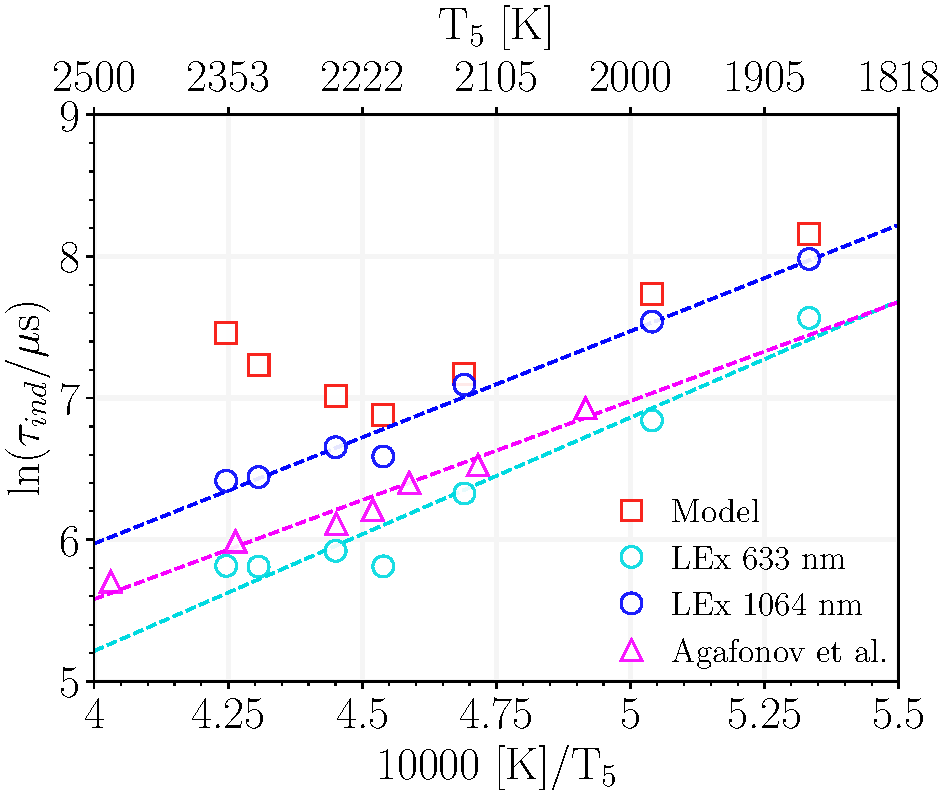
\includegraphics[width=0.65\textwidth]{Figures/Results/Paper3/tau_inc_1064_633.pdf}
	\caption[The predicted soot induction time, $\tau_{ind}$, compared with light extinction measurements at 633~nm and 1064~nm, and with the data from Agafonov. The dashed line is the Arrhenius fit to the measurements.]{The predicted soot induction time, $\tau_{ind}$, compared with light extinction measurements at 633~nm and 1064~nm, and with the data from Agafonov et al.~\citep{agafonov2008soot}. The dashed line is the Arrhenius fit to the measurements.}
	\label{fig:tau_inc_1064_633} 
\end{figure}

The soot induction time ($\tau_{ind}$) is defined as the time extinction level exceeds the noise floor, and it provides a measure of the earliest detectable soot mass and avoid effects of pressure gradients at later times. The noise floor is $f_vE(m) = 2\times10^{-9}$, or $f_v$$\approx$8~ppb (set by beam steering effects). Fig.~\ref{fig:tau_inc_1064_633} demonstrates the predicted $\tau_{ind}$ along with the measurements at 1064~nm and 633~nm that closely follow an Arrhenius-like behavior, expressed as $\tau_{ind} = A_{ind}\exp\left(E_{ind}/{RT}\right)$~\citep{agafonov2008soot}, where $E_{ind}$ is defined as the activation energy of soot inception. The value of $E_{ind}$ is $\approx$130~kJ for both wavelengths, consistent with the range suggested in the literature~\citep{eremin2012formation}, but 1064~nm measurements result in longer induction times. $\tau_{ind}$ obtained from 633~nm measurements are in agreement with the measurements by Agafonov et al.~\citep{agafonov2008soot} for 5\%~CH$_4$ using the same wavelength. The observed difference in $\tau_{ind}$ between two wavelengths is due to higher absorbance at 633~nm, which has been attributed to the non-negligible contribution of large PAHs to absorption at 633~nm~\citep{zerbs2009influence}. In fact, Migliorini et al.~\citep{migliorini2011investigation} showed that the absorption of gaseous species extends up to 700~nm. However, PAHs smaller than circumcoronene ($\mathrm{C_{54}H_{10}}$) are not likely to absorb in wavelengths above 550~nm~\citep{bejaoui2014laser}. 

The model closely reproduces the experimental trends in the low-to-mid temperature range (1800~K-2200~K), but deviates from the measurements for T$_5$$>$2200~K. In fact, the model predicts an inverse temperature dependence for $\tau_{ind}$ relative to PAH concentration, reaching a minimum near the temperature of maximum PAH abundance ($\approx$2200~K) and increasing at higher temperatures where PAH concentrations decline. The carbon yield at $\tau_{ind}$ is close to 0.1\% for T$_5$$\ge$1984~K. The analysis of simulations results at $\tau_{ind}$ suggests that inception accounts for 4.5\%-6.7\% of total soot mass, while the contribution of PAH adsorption decreases from 88\% at T$_5$=1875~K and 1984~K to 50\% at 2355~K. Therefore, the majority of carbon mass at $\tau_{ind}$ originates from precursors that exhibit a bell-shaped temperature dependence. Further analysis suggests that carbonization prolongs the induction time by suppressing HACA rates, but does not alter the temperature dependence of $\tau_{ind}$ (Fig.~\ref{fig:carb_effect_on_tau_inc}). Additional simulations were conducted to assess the sensitivity of $\tau_{inc}$ to precursor selection, in which individual PAHs in the CRECK mechanism were treated separately as the sole precursor. All PAHs produced a similar inverted bell-shaped temperature dependence of $\tau_{inc}$, as shown in Fig.~\ref{fig:tau_inc_1064_633}.







\begin{figure}[!t]
	\centering
	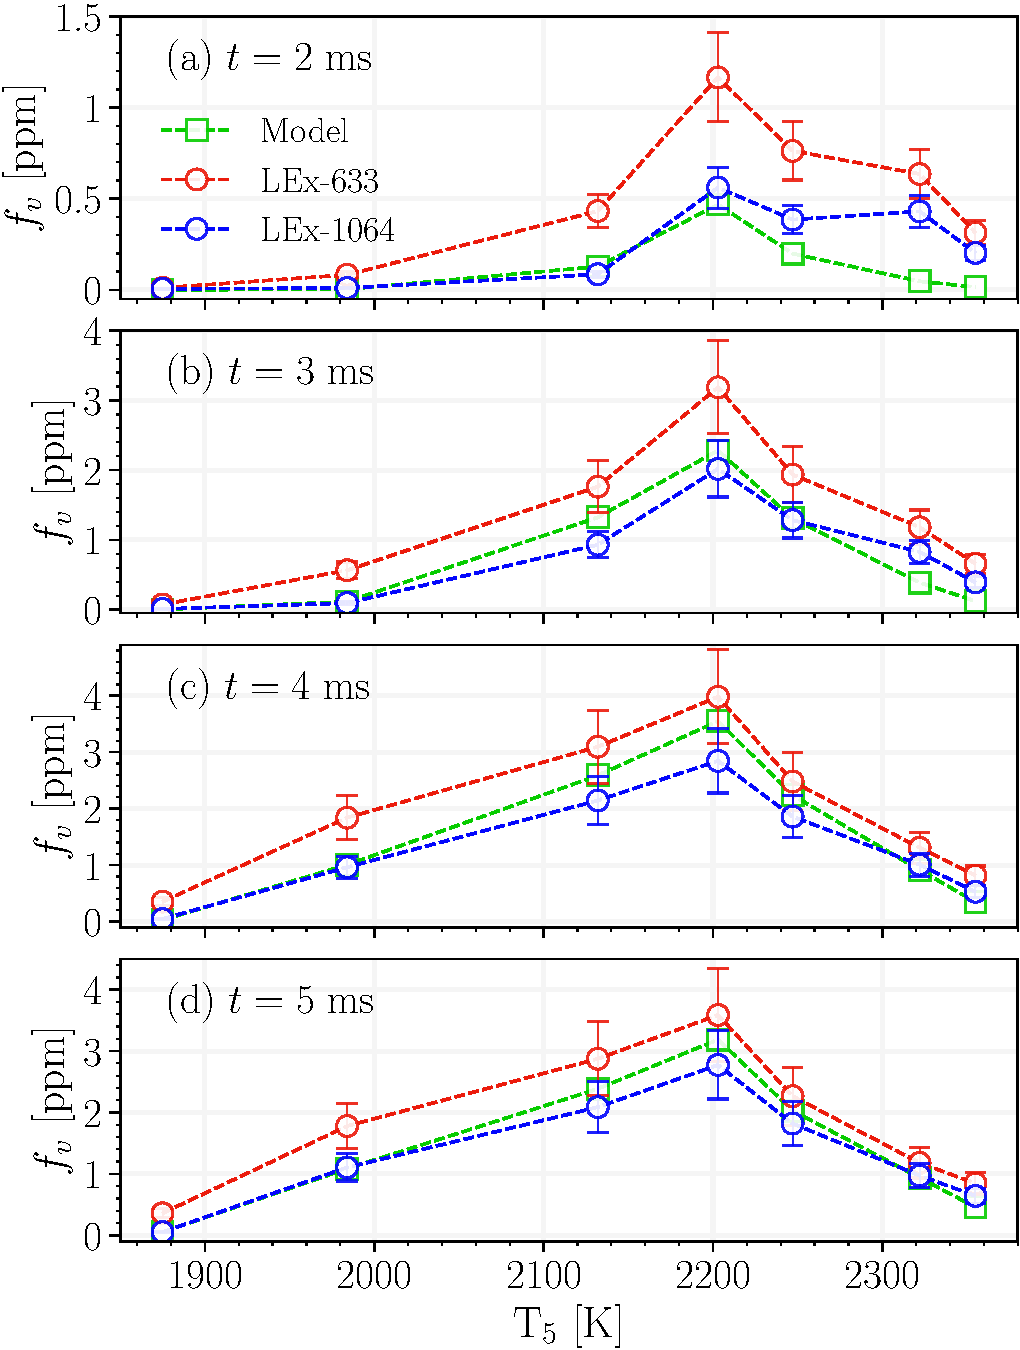
\includegraphics[width=0.65\textwidth]{Figures/Results/Paper3/fv_allconds_sampled_1064_633.pdf}
	\caption{The soot volume fraction, $f_v$, from light extinction at $\lambda=633$~nm sampled at 2~ms (a), 3~ms (b), 4~ms (c), and 5~ms and compared with the simulation results for $\mathrm{T_5}=1875$, 1984, 2132, 2203, 2247, 2355~K. Errors bars indicate experimental uncertainty due to variability in $E(m)$, and the dashed line is added to show the trends.}
	\label{fig:fv_allcases_1064_633} 
\end{figure}

As shown in Fig.~\ref{fig:fv_allcases_1064_633}, a bell-shaped temperature dependence of $f_v$ is observed in the light extinction measurements at 633~nm and 1064~nm at 2, 3, 4, and 5~ms. As discussed earlier, larger $f_v$ values are inferred at 633~nm across the studied T$_5$ range due to stronger absorption at this wavelength compared to 1064~nm. The temperature dependence of $f_v$ is primarily governed by that of soot precursors (Fig.~\ref{fig:precursors_temp_nosoot}) and evolves with time without significant changes in its overall shape, with the peak remaining consistently at T$_5$=2203~K. The model reproduces this temperature dependence in close agreement with the measurements. However, at 2~ms, the model noticeably underpredicts $f_v$ for T$_5$$>$2203~K, consistent with the overestimation of induction time in this temperature range. This discrepancy may be attributed to missing chemical pathways for PAH formation at high temperatures, which would otherwise accelerate inception and PAH adsorption~\citep{wang2024revisit}.



\begin{figure}[!t]
	\centering
	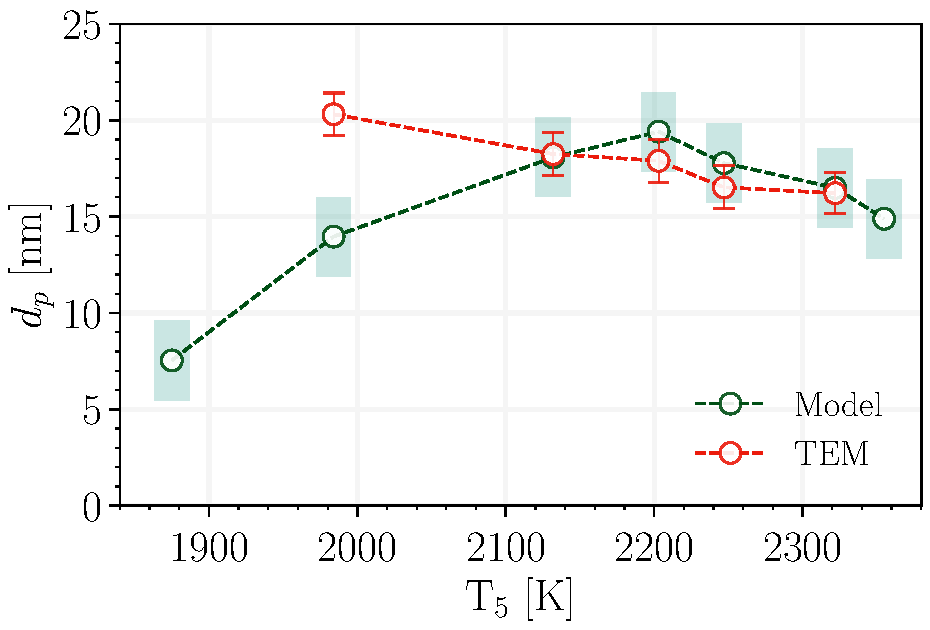
\includegraphics[width=0.7\textwidth]{Figures/Results/Paper3/dp_allconds_sampled.pdf}
	\caption{The final primary particle diameter, $d_p$, from TEM measurements compared with the model predictions.}
	\label{fig:dp_allconds_sampled} 
\end{figure}

Fig.~\ref{fig:dp_allconds_sampled} reveals a significant discrepancy between the predicted and measured temperature dependence of $d_p$. While the TEM measurements exhibit a decreasing trend with increasing T$_5$, the model predicts a bell-shaped profile similar to that of $f_v$, with a peak at 2203~K. No data point was obtained for TEM at T$_5$=1875~K because the collected particles appear as compact carbonaceous lumps with poorly defined boundaries between primary particles rather than chain-like aggregates (Fig.~\ref{fig:tem1875}), which makes the identification of individual primary particles by visual inspection highly uncertain. Nevertheless, some identifiable structures are close to 30~nm, supporting the consistently decreasing trend in $d_p$ inferred from the TEM measurements.

The significant underprediction of $d_p$ at 1984~K, despite the close agreement in the predicted and measured $f_v$ time histories (Fig.~\ref{fig:fv_growth_inception_dpm_timehis_comp}a), can be attributed to the coalescence of primary particles, which increases $d_p$ but is not accounted for in the model. Higher temperatures promote the formation of turbostratic graphite-like order, which inhibits complete merging of particles~\citep{johansson2017evolution}. At the same time, coalescence alters particle surface area and therefore affects surface growth via HACA, which in turn influences $f_v$ predictions. 

In addition, condensation of residual aromatic species beyond 7.5~ms may further contribute to larger primary particle sizes. An upper limit for the increase in $d_p$ was estimated for all conditions by assuming that (i) all residual species containing six or more carbon atoms, equivalent to benzene and larger species, are converted to soot and (ii) the total number of primary particles ($N_{pri}$) remains constant. The revised $d_p$ was calculated as~\citep{adib2026omnisoot}:

\begin{equation}
	d_{p} = \left(\frac{6W_{carbon}}{\pi \rho_{soot}} \frac{C_{tot}+C_{6\ge}}{N_{pri}\cdot Av} \right)^{1/3},
	\label{eqn:d_p}
\end{equation}
where $C_{tot}$ is the total carbon mass of soot gained through surface growth mechanisms, and $C_{6\ge}$ is the total carbon mass in benzene and larger species. Under these assumptions, $d_p$ increases to 25.6~nm at 1875~K from 7.5~nm and to 16.6~nm at 1984~K from 14~nm, whereas the increase at higher T$_5$ remains below 1~nm (Fig.~\ref{fig:dp_allconds_sampled_ext}) resulting in a decreasing temperature dependence similar to the profile obtained from TEM measurements.


\begin{figure}[!t]
	\centering
	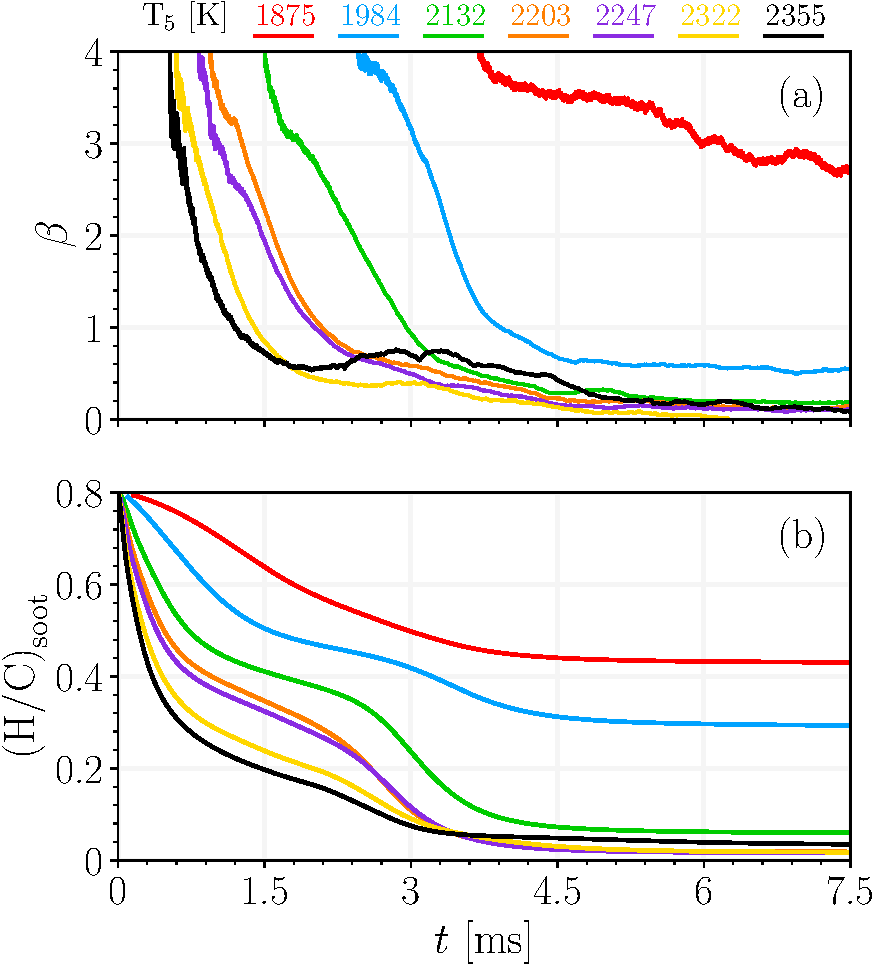
\includegraphics[width=0.7\textwidth]{Figures/Results/Paper3/htoc_extio_all_cases.pdf}
	\caption{The evolution of (a) maturity index, $\beta$, obtained from extinction measurements at 633~nm and 1064~nm, and (b) the predicted H/C ratio of soot particles at various T$_5$.}
	\label{fig:htoc_extio_all_cases} 
\end{figure}


Fig.~\ref{fig:htoc_extio_all_cases}a depicts the maturity index, $\beta$, inferred from the extinction ratio at 633~nm and 1064~nm~\citep{yon2021revealing} as

\begin{equation}
\beta= \mathrm{ln}\left(\frac{E(m,\lambda_{633})}{E(m,\lambda_{1064})}\right)
/\mathrm{ln}\left(\frac{\lambda_{1064}}{\lambda_{633}}\right).
\label{eqn:d_p}
\end{equation}

The progression from high to low $\beta$ with increasing time reflects the transformation of soot from disordered PAH clusters to particles with concentric graphitic layers. This structural evolution is accompanied by chemical carbonization, manifested as a decrease in the hydrogen-to-carbon (H/C) ratio due to dehydrogenation~\citep{cepeda2025effect}. As shown in Fig.~\ref{fig:htoc_extio_all_cases}b, $\beta$ exhibits strong qualitative agreement with the predicted H/C ratio of soot particles in both time history and temperature dependence. In all cases, both quantities show an initial rapid decline whose rate increases with T$_5$, followed by a slower decrease toward asymptotic values $\approx$0, indicating increasing soot maturity and weak spectral dependence. Notably, the $\beta$ and H/C profiles at 1875~K and 1984~K converge to higher final values than those at T$_5 \ge 2132$~K, indicating incomplete carbonization and lower structural ordering under these conditions. In contrast, the higher-T$_5$ cases approach similar late-time values, suggesting that once a threshold temperature is exceeded, soot maturity becomes relatively insensitive to further increases in T$_5$ within the studied range.